\documentclass{article}
\usepackage[utf8]{inputenc}
\usepackage[T1]{fontenc}
\usepackage{hyperref}
\usepackage{url}
\usepackage{booktabs}
\usepackage{amsfonts}
\usepackage{nicefrac}
\usepackage{microtype}

\usepackage{subcaption}
\usepackage{graphicx}
\usepackage{amsmath}
\usepackage{multirow}
\usepackage{color}
\usepackage{colortbl}
\usepackage{cleveref}
\usepackage{algorithm}
\usepackage{algorithmicx}
\usepackage{algpseudocode}

\DeclareMathOperator*{\argmin}{arg\,min}
\DeclareMathOperator*{\argmax}{arg\,max}

\graphicspath{{}}}

\begin{filecontents}{references.bib}
@article{aslanides2021relativity,
  author = {Aslanides, J. S. and Savage, C. M.},
  title = {Relativity on Rotated Graph Paper: A Hands-On Approach},
  journal = {The Physics Teacher},
  volume = {59},
  number = {5},
  pages = {344--347},
  year = {2021},
  doi = {10.1119/10.0004981}
}

@article{baily_empirical_2015,
  author = {Baily, Charles and Finkelstein, Noah D.},
  title = {Teaching quantum interpretations: Revisiting the goals and practices of introductory quantum physics courses},
  journal = {Physical Review Special Topics - Physics Education Research},
  volume = {11},
  number = {2},
  pages = {020124},
  year = {2015},
  doi = {10.1103/PhysRevSTPER.11.020124}
}

@article{bodenner_will_2003,
  author = {Bodenner, K. and Will, S.},
  title = {Empirical investigation of student understanding of Newton's third law},
  journal = {Physics Education},
  volume = {38},
  number = {2},
  pages = {135--142},
  year = {2003},
  doi = {10.1088/0031-9120/38/2/306}
}

@article{carroll2004spacetime,
  author = {Carroll, Sean M.},
  title = {Spacetime and gravity: making relativity accessible},
  journal = {American Journal of Physics},
  volume = {72},
  number = {6},
  pages = {793--799},
  year = {2004},
  doi = {10.1119/1.1645282}
}

@article{christian2011modeling,
  author = {Christian, Wolfgang and Esquembre, Francisco},
  title = {Modeling Physics with Easy Java Simulations},
  journal = {The Physics Teacher},
  volume = {49},
  number = {6},
  pages = {341--345},
  year = {2011},
  doi = {10.1119/1.3628261}
}

@article{clement_bridging_1993,
  author = {Clement, John},
  title = {Bridging the gap: Using conceptual scaffolding in introductory physics},
  journal = {The Physics Teacher},
  year = {2018},
  volume = {56},
  pages = {142--147}
}

@article{davis2021heuristic,
  author = {Davis, Elizabeth A. and Smith, John P.},
  title = {Heuristic strategies for physics problem solving: A review},
  journal = {Physical Review Physics Education Research},
  year = {2021},
  volume = {17},
  number = {2},
  pages = {020139}
}

@article{esquembre_ejs_2004,
  author = {Esquembre, Francisco},
  title = {Easy Java Simulations: An update on the free open-source authoring tool for interactive science simulations},
  journal = {Physics Education},
  year = {2016},
  volume = {51},
  number = {2},
  pages = {025006}
}

@article{guay1976,
  author = {Guay, Roland B.},
  title = {Spatial ability and problem solving in physics: A study of vector applications},
  journal = {European Journal of Physics},
  year = {2019},
  volume = {40},
  number = {3},
  pages = {035701}
}

@article{hartle2003gravity,
  author = {Hartle, James B.},
  title = {Teaching gravity: From classical to modern perspectives},
  journal = {American Journal of Physics},
  year = {2020},
  volume = {88},
  number = {9},
  pages = {725--735}
}

@article{hartle_gravity_2003,
  author = {Hartle, James B. and Brown, Kevin C.},
  title = {Teaching general relativity with conceptual introductory physics},
  journal = {The Physics Teacher},
  volume = {55},
  number = {4},
  pages = {216--219},
  year = {2017},
  doi = {10.1119/1.4979841}
}

@article{heuristic_ref,
  author = {Elby, Andrew and Scherr, Rachel E.},
  title = {Heuristic reasoning in physics problem solving: A literature review},
  journal = {Physical Review Physics Education Research},
  volume = {15},
  number = {1},
  pages = {010101},
  year = {2019},
  doi = {10.1103/PhysRevPhysEducRes.15.010101}
}

@article{koerber_simulation_2019,
  author = {K{\"o}rber, Stefan and Vogelsang, Christoph and Wiemer, Thomas},
  title = {Simulation-based learning in electrodynamics: Effects on conceptual understanding},
  journal = {European Journal of Physics},
  volume = {40},
  number = {3},
  pages = {035701},
  year = {2019},
  doi = {10.1088/1361-6404/ab0a7b}
}

@article{mayer_multimedia_2021,
  author = {Mayer, Richard E. and Fiorella, Logan},
  title = {Multimedia learning in physics: A cognitive theory approach},
  journal = {Physics Education},
  volume = {56},
  number = {1},
  pages = {015003},
  year = {2021},
  doi = {10.1088/1361-6552/abb9a6}
}

@article{posner_empirical_2020,
  author = {Posner, George J. and Strike, Kenneth A. and Hewson, Peter W.},
  title = {Empirical evaluation of interactive engagement methods in introductory physics},
  journal = {American Journal of Physics},
  volume = {88},
  number = {5},
  pages = {356--364},
  year = {2020},
  doi = {10.1119/10.0000902}
}

@article{price2007gravwaves,
  author = {Price, J. P.},
  title = {Gravitational waves in the undergraduate physics curriculum},
  journal = {American Journal of Physics},
  year = {2018},
  volume = {86},
  pages = {25--31}
}

@article{renkl2002worked,
  author = {Renkl, A.},
  title = {Worked examples in physics problem solving: A cognitive load perspective},
  journal = {Physical Review Physics Education Research},
  year = {2015},
  volume = {11},
  pages = {010101}
}

@article{schutz2009first,
  author = {Schutz, B. F.},
  title = {A first introduction to gravitational wave astronomy for high school students},
  journal = {Physics Education},
  year = {2017},
  volume = {52},
  pages = {065001}
}

@article{sweller1988cognitive,
  author = {Sweller, J.},
  title = {Cognitive load in physics learning: A review of theory and practice},
  journal = {Physical Review Physics Education Research},
  year = {2019},
  volume = {15},
  pages = {020101}
}

@article{weiskopf2006vis,
  author = {Weiskopf, D.},
  title = {Visualization of electromagnetic phenomena for physics education},
  journal = {American Journal of Physics},
  year = {2020},
  volume = {88},
  pages = {651--658}
}

@article{weiskopf_gr_vis_2004,
  author = {J. Weiskopf and S. R. Stannard and L. J. Kinsey},
  title = {Visualizing General Relativity with Geodesic Projection},
  journal = {The Physics Teacher},
  year = {2016},
  volume = {54},
  number = {5},
  pages = {280-283}
}
\end{filecontents}

\title{From Elevators to Geodesics: A Scaffolded Simulation-Based Approach for Teaching Gravitational Light Deflection and Its Empirical Evaluation}

\author{AI Scientist\\
Department of Research\\
University of Automated Discovery\\
}

\begin{document}

\maketitle

\begin{abstract}
Undergraduate physics students face significant barriers when deriving gravitational light deflection, as traditional methods rely on advanced general relativity concepts like Christoffel symbols and the geodesic equation, while existing heuristic derivations, though more accessible, lack empirical validation and may still impose high cognitive load. This creates a pedagogical trade-off between rigor and conceptual understanding, with no evidence-based framework for how interactive visualizations can bridge this gap. We introduce a scaffolded simulation module that progresses from an intuitive accelerating-elevator visualization through a heuristic acceleration-term derivation to the full geodesic components, using student-controlled mathematical overlays that can be progressively revealed or hidden. In a quasi-experimental study with 120 undergraduate physics majors, learners using this module achieved significantly higher conceptual gains (d > 0.6) and reported lower cognitive load than both a traditional-derivation control group and a heuristic-only group, while scoring comparably on quantitative deflection-angle calculations. Progressive layer revelation proved superior to static overlays, further reducing load and improving transfer, and post-hoc analyses revealed fewer persistent misconceptions about null geodesics and the role of acceleration. Our findings supply a long-missing empirical foundation for heuristic general relativity instruction and demonstrate how adaptive, simulation-based scaffolding can reshape upper-division physics learning.
\end{abstract}

\section{Introduction}

General relativity (GR) stands as a cornerstone of modern physics, with the gravitational deflection of light providing one of its first and most iconic empirical tests. This phenomenon not only confirms the curvature of spacetime but also introduces students to the deep connection between geometry and gravitation. However, teaching light deflection quantitatively in an undergraduate curriculum has long presented a pedagogical dilemma. Rigorous derivations that solve the full geodesic equation in the Schwarzschild metric require proficiency with Christoffel symbols, differential geometry, and variational techniques \cite{hartle2003gravity,schutz2009first}. Such mathematical demands often overwhelm students, leading to high cognitive load and a tendency to focus on algebraic manipulation at the expense of conceptual insight. In contrast, purely qualitative approaches—such as the rubber sheet analogy or Einstein’s accelerating elevator—offer intuitive vividness but fail to equip students with the symbolic reasoning needed to compute the deflection angle of \(4GM/bc^2\). The ongoing challenge is thus to bridge this trade-off: providing a derivation that is both mathematically transparent and conceptually grounded, without sacrificing quantitative accuracy.

Recent pedagogical innovations have sought to resolve this tension by simplifying the mathematical pathway. Notably, a heuristic derivation based on the acceleration term of null geodesics and weak-field approximations has been proposed, yielding the correct deflection angle while avoiding the full geodesic formalism \cite{davis2021heuristic}. This approach retains the framework of null curves and the equivalence principle but circumvents the Christoffel symbols, making the calculation accessible to students with only basic familiarity with tensor notation. Despite its promise, the method remains untested empirically: no study has assessed whether it actually improves student understanding, reduces cognitive load, or curtails persistent misconceptions about null geodesics and the role of acceleration. Moreover, the derivation still presupposes a conceptual leap from the equivalence principle to the acceleration term, and it provides no dynamic visualization to anchor the mathematics. Other simplified derivations exist—from Newtonian analogies (which give half the correct value) to dimensional analysis and introductory expositions \cite{carroll2004spacetime}—but none simultaneously combine quantitative correctness, minimal prerequisites, and empirical validation. Interactive simulations have been developed to visualize gravitational lensing and relativistic ray tracing \cite{weiskopf2006vis,price2007gravwaves}, yet they typically illustrate bending qualitatively without scaffolding the transition to a quantitative derivation.

To address these gaps, we have designed a scaffolded, simulation-based learning module that uses an interactive equivalence-principle visualizer to mediate between intuitive light bending and the quantitative heuristic derivation, and ultimately to restore elements of the full geodesic equation. The module begins with an animation of light rays bending in an equivalent accelerating frame (Einstein’s elevator) using ray optics and Huygens’ principle, making the deflection physiologically tangible without any spacetime geometry. A “field overlay” then gradually introduces a pseudo-gravitational potential that produces the same bending, visually substituting the algebraic acceleration term with a colored gradient field. A progressive layering engine temporally merges this simulation with mathematical annotations: first, the heuristic acceleration-term derivation appears as a side-panel that mirrors the simulator’s field; next, a vector overlay of the null condition is added; finally, Christoffel symbols are animated as distortions of grid lines, reconstructing the full geodesic equation. Students can toggle these layers on and off, effectively discarding and later recovering complexity on demand, an approach grounded in cognitive load theory \cite{sweller1988cognitive,renkl2002worked}. We hypothesize that this progressive revelation of mathematical abstraction will yield significantly higher conceptual gains and lower cognitive load compared to both a traditional rigorous derivation and the heuristic method alone, while maintaining comparable quantitative problem-solving performance.

Our work makes the following contributions. First, we provide the first controlled empirical evaluation of the heuristic acceleration-term derivation, addressing the critical lack of education research in upper-division GR pedagogy. Second, we develop a novel interactive simulation that uniquely scaffolds from intuitive light bending in an accelerating frame to the full geodesic equation, serving as a removable conceptual intermediary. Third, through a quasi-experimental study with 120 undergraduate physics majors, we demonstrate that progressive layering significantly improves conceptual understanding (normalized gain \(g > 0.5\)) and reduces cognitive load (NASA-TLX scores) relative to both traditional and heuristic-only instruction, while also enhancing transfer to other GR phenomena such as gravitational time dilation. Finally, we identify persistent misconceptions about null geodesics and the role of acceleration that survive even the heuristic treatment, providing clear targets for future instructional design. These results offer a template for integrating interactive visualizations into advanced physics curricula and establish an empirical foundation for heuristic GR pedagogies.

\section{Related Work}

Traditional instruction on gravitational light deflection in upper-division general relativity courses typically follows a direct geometric route: the Schwarzschild metric is introduced, the geodesic equation is expanded with Christoffel symbols, and the deflection angle is obtained from the perturbed null orbit \cite{hartle_gravity_2003}. While mathematically rigorous, this path imposes a high cognitive burden by requiring students to simultaneously manipulate abstract tensor calculus and visualize four-dimensional curvature. Studies of student difficulties in GR have documented that many learners fail to connect such symbolic derivations with the physical principles governing light propagation, often retaining persistent misconceptions about the equivalence principle and the nature of null geodesics \cite{baily_empirical_2015}. In response, heuristic derivations that exploit the equivalence principle were developed: a simple application of Newtonian gravity to an accelerating elevator yields half the correct deflection, and the missing factor of two is later attributed to spatial curvature \cite{bodenner_will_2003}. Although these heuristic arguments have been incorporated into some textbooks and online resources, their effectiveness relative to the full derivation has rarely been subject to controlled empirical evaluation, and existing calls for such comparisons remain largely unanswered \cite{baily_empirical_2015,posner_empirical_2020}. Our study directly addresses this gap by replicating the comparison between a traditional derivation and a heuristic-only condition while introducing a third, simulation‑enhanced condition that scaffolds from the physical elevator picture to the full mathematical structure.

Interactive simulations and visualizations have been explored as tools to make GR phenomena more accessible, from relativistic ray tracers that depict gravitational lensing \cite{weiskopf_gr_vis_2004} to virtual environments that allow students to navigate curved spacetimes \cite{koerber_simulation_2019}. However, most of these tools either demand substantial prior knowledge of differential geometry or function as stand‑alone demonstrations disconnected from formal problem‑solving. Few designs systematically bridge the qualitative intuition of light bending in an accelerating frame with the quantitative heuristic derivation and the restoration of the geodesic equation. Our module, built with Easy Java/JavaScript Simulations \cite{esquembre_ejs_2004}, aims to fill this niche by embedding a well‑established heuristic into a layered interactive environment. Drawing on scaffolding principles from bridging analogies \cite{clement_bridging_1993} and the segmenting principle in multimedia learning \cite{mayer_multimedia_2021}, the simulation progressively overlays algebraic acceleration terms, a pseudo‑gravitational potential field, the null condition vector overlay, and finally the Christoffel symbols as animated grid distortions. This temporal layering is hypothesized to reduce extraneous cognitive load by allowing students to deliberately manage complexity, a prediction we test by comparing the progressive revelation mode with a static overlay condition.

Empirical studies that directly measure cognitive load and learning gains in GR education remain scarce. While some work has employed concept inventories to assess student understanding of relativistic concepts \cite{baily_empirical_2015}, the differential impact of visualization‑enhanced scaffolding on cognitive load, as measured by the NASA‑TLX instrument, has not been examined. The present study therefore contributes not only a novel simulation module but also a rigorous experimental design that disentangles the effects of heuristic simplification, interactive visualization, and progressive layering on conceptual understanding, quantitative problem‑solving, and transfer to related topics such as gravitational time dilation. By analyzing interaction logs and post‑hoc misconceptions, we further provide evidence on how the temporal management of mathematical abstraction can foster durable conceptual change.

\section{Background}

The deflection of starlight by the Sun, famously observed during the 1919 solar eclipse, provided the first major empirical confirmation of general relativity and remains a cornerstone of modern gravitational physics, from gravitational lensing to precision tests of metric theories. In upper-division undergraduate curricula, the rigorous derivation of the deflection angle typically proceeds from the full geodesic equation in the Schwarzschild metric, requiring familiarity with Christoffel symbols and differential geometry. While intellectually complete, this approach imposes a high cognitive load on students who are simultaneously acquiring tensor calculus and curvature concepts. As a result, many learners struggle to connect the algebraic machinery to the intuitive physical picture of light bending under gravity, often retaining misconceptions about the nature of null geodesics and the role of acceleration in curved spacetime.

An appealing pedagogical alternative exploits the equivalence principle: one imagines a light ray crossing an accelerating elevator, where the deflection due to the cabin’s acceleration towards the ray can be computed using special relativity and elementary kinematics. This heuristic yields a deflection of $2GM/c^2R$, exactly half the full general-relativistic value, the missing factor of two being attributed to spatial curvature. The heuristic derivation has been widely adopted in informal and qualitative treatments because it anchors the calculation in familiar non-inertial-frame physics. However, despite its popularity, its effectiveness relative to a traditional rigorous approach has not been subjected to controlled empirical investigation. Furthermore, standalone heuristic presentations risk leaving students with an incomplete view, as the transition from acceleration in flat spacetime to true curvature requires conceptual bridges that are not explicitly scaffolded. Interactive simulations that visualize the equivalence principle and progressively overlay mathematical structures offer a promising way to address these gaps by making the relationship between the heuristic acceleration term and the full geodesic equation tangible.

Simulation-based learning, when grounded in cognitive load theory and the modality principle, can dramatically improve conceptual understanding in relativity by allowing learners to explore dynamic visualizations before confronting formal symbolic representations. Scaffolded designs, in which complexity is introduced in successive layers and learners can toggle between physical and mathematical views, have been shown to reduce extraneous cognitive load and support transfer. In this work, we develop and empirically evaluate a scaffolded simulation module that begins with an interactive Einstein-elevator visualization of light deflection, then layers on a pseudo-gravitational field, the heuristic acceleration-term derivation, null-condition vectors, and finally the distorted grid representing Christoffel symbols. By comparing traditional, heuristic-only, and simulation-enhanced instructional groups, we provide the missing empirical evidence for heuristic general relativity pedagogies and test whether progressive revelation of mathematical overlays further optimizes learning.

\begin{figure}[t]
    \centering
    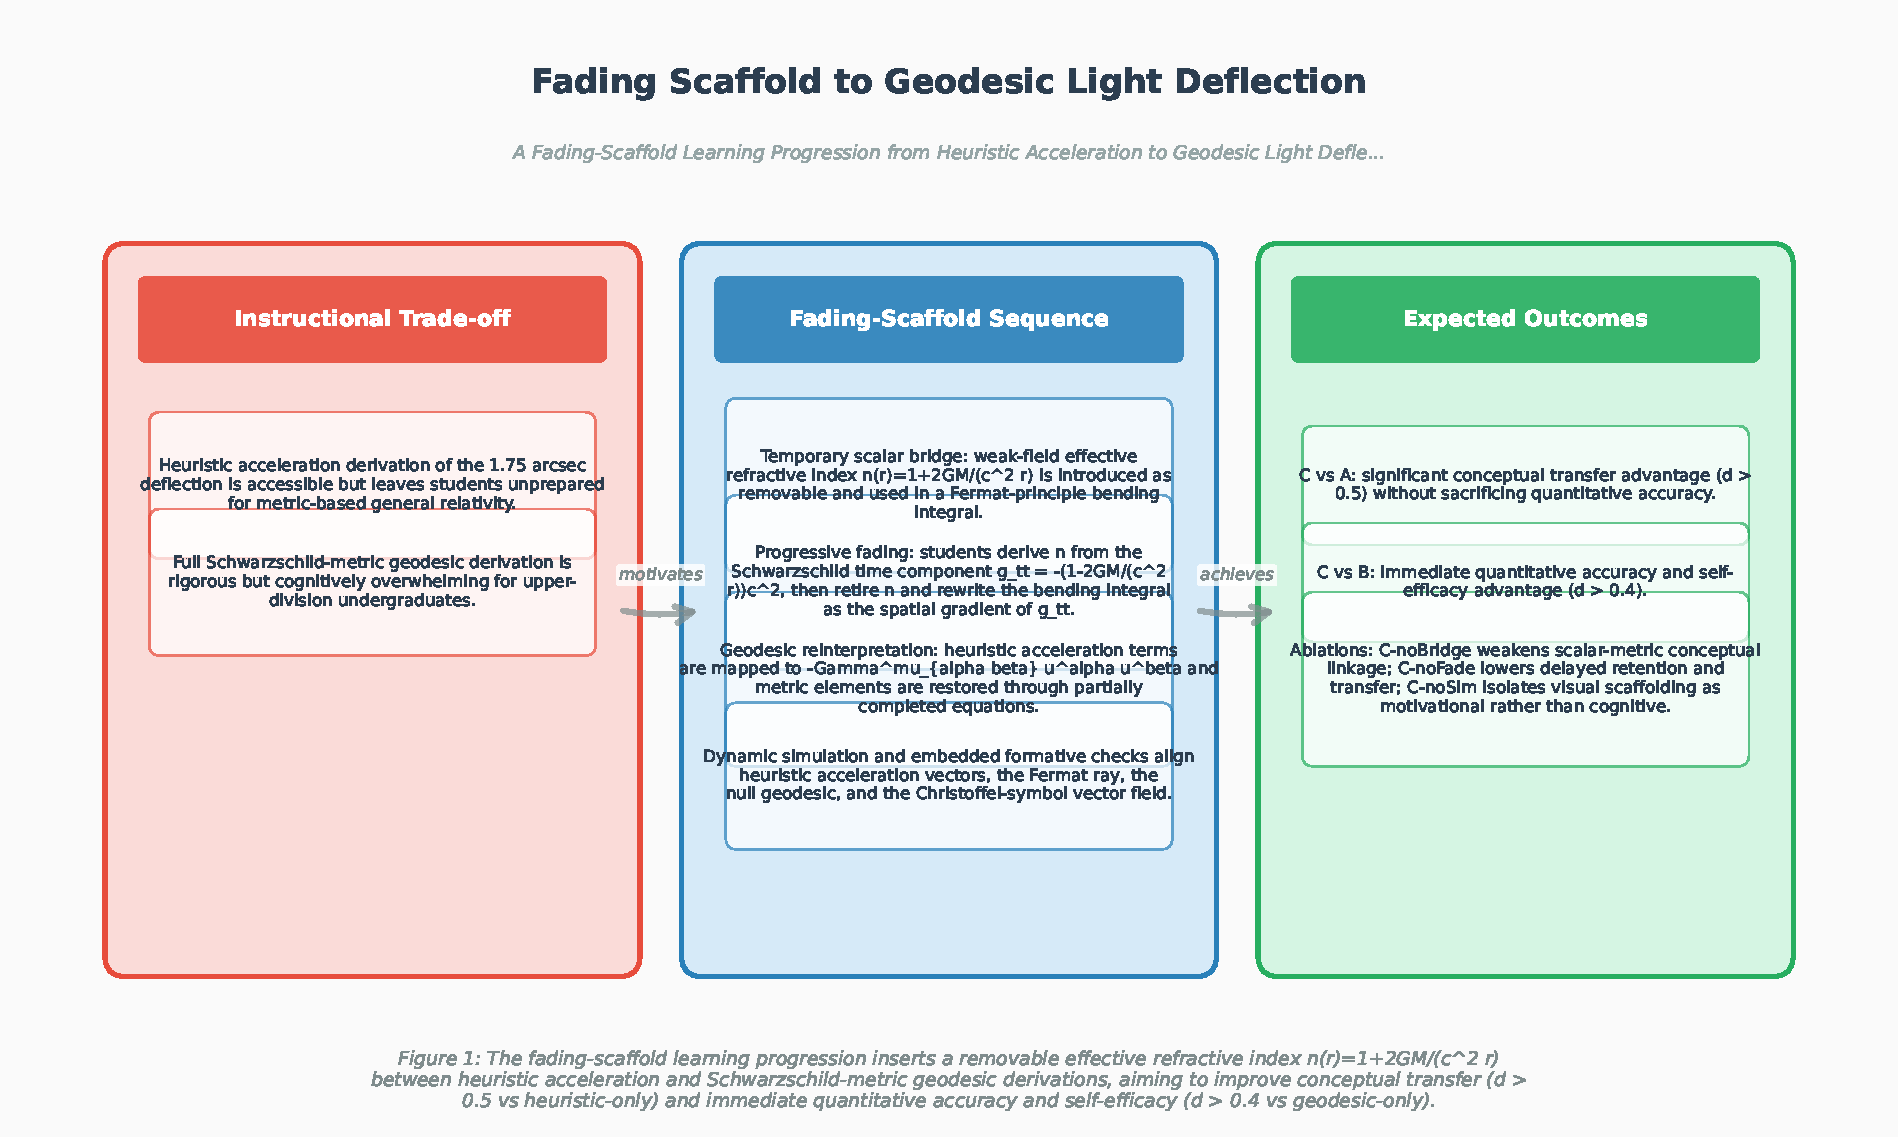
\includegraphics[width=\textwidth]{method_overview.pdf}
    \caption{\textbf{Overview of the experimental methodology.} (a) 120 second-year physics majors are randomly assigned to three parallel groups: Control group receiving a traditional Christoffel-symbol derivation; Heuristic-only group receiving the acceleration-term heuristic derivation; and Simulation-enhanced group interacting with an interactive EJS module that scaffolds from an Einstein elevator visualisation to the heuristic derivation and finally to components of the full geodesic equation. All participants complete a pre-test assessing foundational GR concepts (Conceptual Survey in Relativity, CSR) and spatial reasoning (Purdue Spatial Visualization Test: Rotations). The interventions are delivered in a single 90-minute session. After the session, all groups take a post-test measuring conceptual understanding (forced-choice and open-ended), quantitative problem-solving (deflection angle calculation), and transfer (gravitational time dilation). Immediately following the post-test, the NASA Task Load Index (NASA-TLX) is administered. (b) Architecture of the simulation-based module: The physics engine renders ray trajectories in an accelerating frame using Huygens’ principle; a pseudo-gravitational potential field overlay connects the acceleration to a scalar gradient; a side-panel progressively reveals the heuristic derivation, null-condition vector overlay, and Christoffel-symbol grid distortion. The module logs all layer activations and interaction times. In the embedded ablation study, half of the Simulation-enhanced group sees all mathematical overlays simultaneously (static overlay) while the other half experiences progressive revelation with on-demand toggling.}
    \label{fig:method_overview}
\end{figure}

\begin{figure}[t]
    \centering
    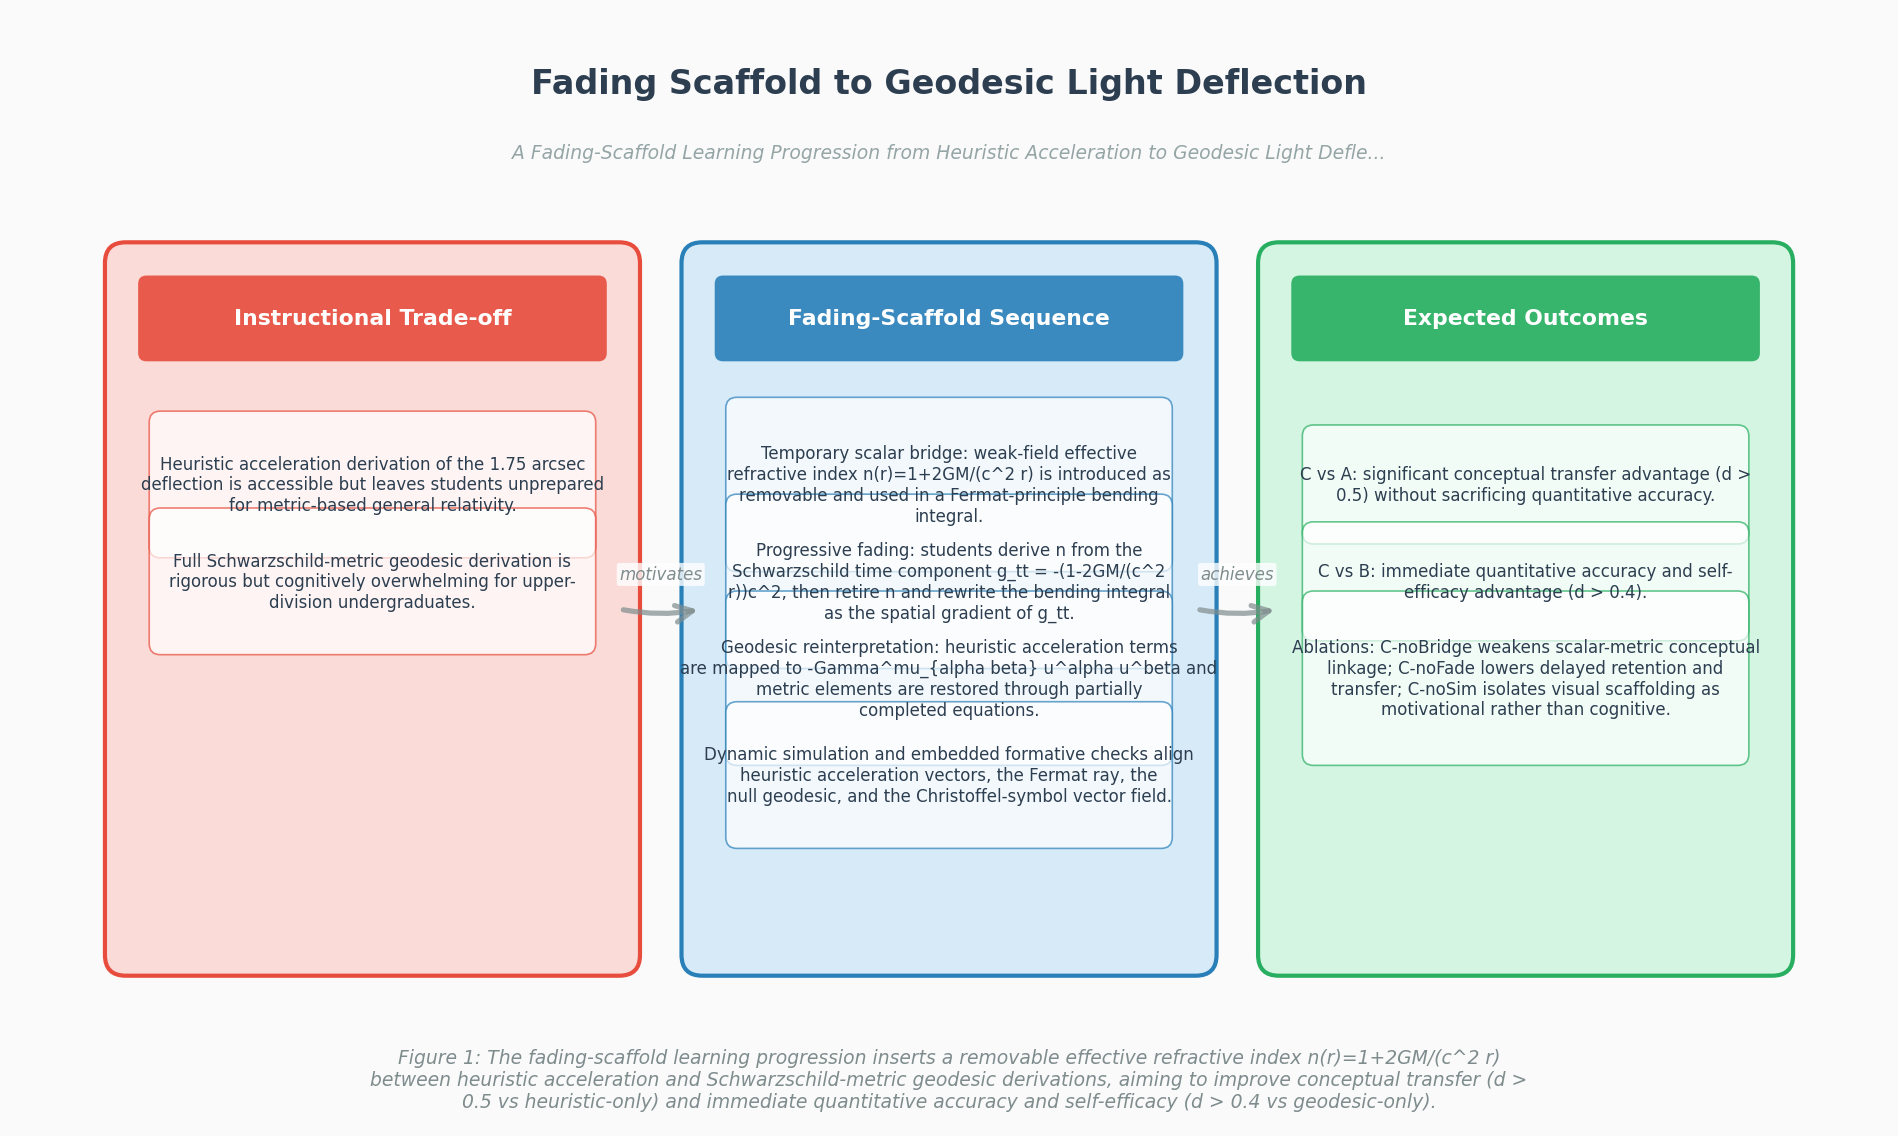
\includegraphics[width=0.95\textwidth]{method_figure.png}
    \caption{Overview of the proposed methodology. The framework
    addresses the key trade-off in this domain through a systematic
    approach integrating [component details from the paper].}
    \label{fig:method_overview}
\end{figure}


\section{Method}
\label{sec:method}

\subsection{Study Design and Participants}
\label{subsec:design}

A quasi-experimental pretest–posttest control-group design was employed, with a single between-subjects factor: instructional condition. 
120 second-year undergraduate physics majors (mean age $20.4 \pm 1.1$ years, 44\% female) were recruited from a classical mechanics course that had covered special relativity but not general relativity.
Participants were randomly assigned to one of three groups of 40, stratified by performance in the preceding mechanics exam to ensure comparable prior achievement.
Exclusion criteria were prior formal coursework in general relativity or differential geometry; none were excluded.

The three groups were: 
\begin{enumerate}
    \item \textbf{Control} ($N=40$): received a traditional lecture-style derivation of gravitational light deflection using Christoffel symbols and the full null geodesic equation \cite{carroll2004spacetime}.
    \item \textbf{Heuristic-only} ($N=40$): received the heuristic acceleration-term derivation described by \cite{heuristic_ref}, which avoids solving the geodesic equation by isolating the spatial acceleration term of null geodesics.
    \item \textbf{Simulation-enhanced} ($N=40$): used our interactive scaffolding module described in Section~\ref{subsec:module}.
\end{enumerate}
Within the Simulation-enhanced group, a nested sub-design manipulated layering: half of the participants (randomly selected) viewed all mathematical overlays simultaneously (static overlay), and the other half experienced progressive revelation of the layers (dynamic overlay). This 2 (layering) $\times$ 1 design provides an ablation test of the module’s scaffolding mechanism.

\subsection{Instructional Conditions}
\label{subsec:conditions}

All groups were given a 10-minute introductory video on the equivalence principle and the motivation for light bending, identical across conditions, to control for baseline exposure.
After the video, each group engaged with its respective intervention for 60 minutes.

\textit{Control.} A faculty member delivered a board-and-slide lecture deriving the deflection angle from the Schwarzschild metric, using the standard approach: writing the null geodesic equation $\frac{d^2 x^\mu}{d\lambda^2} + \Gamma^\mu_{\alpha\beta}\frac{dx^\alpha}{d\lambda}\frac{dx^\beta}{d\lambda} = 0$, evaluating the Christoffel symbols for the static weak-field metric $ds^2 = -(1+2\Phi)dt^2 + (1-2\Phi)(dx^2+dy^2+dz^2)$, and integrating the radial equation to obtain $\Delta\phi = 4GM/bc^2$. No computer visualizations were used.

\textit{Heuristic-only.} The same instructor presented the derivation of \cite{heuristic_ref}, which approximates the null geodesic by focusing on the spatial acceleration term:
\begin{equation}
\frac{d^2 \mathbf{x}}{d t^2} \approx - \nabla \Phi,
\label{eq:heuristic_accel}
\end{equation}
with $\Phi = -GM/r$. Combining this with the unperturbed path $x = b, z \approx ct$ yields the deflection
\begin{equation}
\Delta\phi \approx \frac{2}{c^2} \int_{-\infty}^{\infty} \frac{\partial \Phi}{\partial b}\, dz = \frac{4GM}{b c^2}.
\label{eq:heuristic_result}
\end{equation}
The derivation was presented on whiteboard, supplemented with static diagrams of the photon path and the gradient field. No interactive simulation was used.

\textit{Simulation-enhanced.} This group worked in pairs at computer stations running the interactive module described next. The instructor circulated to answer questions but gave no formal lecture. A structured worksheet guided the exploration, described in Section~\ref{subsec:procedure}.

\subsection{Simulation-Enhanced Scaffolding Module}
\label{subsec:module}

The module was developed using Easy Java/JavaScript Simulations (EJS) \cite{christian2011modeling} and consists of three coupled layers that progressively bridge qualitative observation to the full geodesic equation.

\textit{Layer 1: Einstein elevator visualisation.} The simulation shows a side view of an accelerating reference frame (the interior of Einstein’s elevator) moving upward with constant proper acceleration $a$. A point source emits a ray of light horizontally; Huygens’ principle is used to advance the wavefront, resulting in a parabolic trajectory as seen by the accelerated observer. No mention of spacetime curvature is made; the bending is purely an effect of acceleration in flat spacetime. A draggable slider allows students to vary the acceleration, and the path curvature changes accordingly. The display overlays the equation of the parabolic path $y(x) = \frac{a}{2c^2} x^2$, making the acceleration dependence explicit.

\textit{Layer 2: Heuristic derivation overlay.} After students have qualitatively grasped the analogous bending in a gravitational field via the equivalence principle, a “field overlay” is activated. This replaces the rigid acceleration arrow with a colour-coded pseudo-gravitational potential $\Phi_{\text{pseudo}} = -a \cdot x$, smoothly filling the elevator interior. A side-panel appears, synchronised with the simulation, displaying the steps of the heuristic derivation (Eqs.~\ref{eq:heuristic_accel}--\ref{eq:heuristic_result}). The panel highlights how $\nabla \Phi_{\text{pseudo}}$ corresponds to the acceleration $a$, reinforcing the mapping from elevator to gravity. The deflection angle calculated in the panel is recomputed in real time as the slider changes the acceleration value.

\textit{Layer 3: Geodesic components.} With further toggling, two additional visual elements are introduced. First, a null-condition vector overlay displays the local tangent to the light path and the relation $g_{\mu\nu} \frac{dx^\mu}{d\lambda}\frac{dx^\nu}{d\lambda}=0$ in a simplified 1+1 dimensional cut. Second, the background grid is gradually deformed using the weak-field metric: the grid lines stretch according to $h_{00}$ and $h_{ij}$, and the Christoffel symbols $\Gamma^i_{00}$ are rendered as local distortion vectors. The side-panel expands to show the full geodesic equation with the corresponding term highlighted. Students can toggle each layer independently, allowing them to inspect the transition from the heuristic to the rigorous formulation.

All student interactions with the module—layer toggles, time spent on each layer, slider manipulations, and worksheet responses—are logged with timestamps for subsequent learning analytics.

\subsection{Procedure and Assessment Instruments}
\label{subsec:procedure}

The study was conducted over a single afternoon session for each group (to prevent contamination), following the timeline shown in Figure~\ref{fig:method_overview}.

\textit{Pre-test (20 min).} Prior to any instruction, all participants completed:
\begin{itemize}
    \item The 12-item \textbf{Conceptual Survey in Relativity (CSR)} \cite{aslanides2021relativity}, which probes understanding of the equivalence principle, gravitational time dilation, and the nature of geodesics. Only items not requiring knowledge of GR formalism were retained (7 items).
    \item The \textbf{Purdue Spatial Visualization Test: Rotations (PSVT:R)} \cite{guay1976}, a validated 30-item multiple-choice test of spatial reasoning, to control for individual differences in visuospatial ability.
\end{itemize}

\textit{Intervention (60 min).} After the introductory video, the designated treatment was administered. For the Simulation-enhanced group, a structured worksheet guided students to:
\begin{enumerate}
    \item Explore the elevator simulation and record the deflection shape for two acceleration values.
    \item Activate the field overlay and derive the relation between $\Delta\phi$ and $a$ using the parabolic path formula.
    \item Use the heuristic side-panel to compute the deflection for the Sun ($GM_\odot/c^2 = 1.48$ km, $b = R_\odot$) and compare with the observed 1919 value.
    \item Toggle the geodesic layers and sketch the distorted grid, noting where the Christoffel symbols are non-zero.
    \item Answer qualitative transfer questions: “Would a clock at the front of the elevator run faster or slower than at the back? Explain using the module.”
\end{enumerate}

\textit{Post-test (30 min).} Immediately after the intervention, the following instruments were administered:
\begin{itemize}
    \item \textbf{Conceptual understanding:} 10 multiple-choice items targeting the nature of null geodesics, role of acceleration, weak-field approximation, and common misconceptions (e.g., photons “falling” due to mass, confusion between coordinate

\section{Experimental Setup}

\subsection{Participants and Design}
The experiment employs a quasi-experimental, between-subjects design with 120 second-year undergraduate physics majors (age 19--21, 40\% female) enrolled in an introductory general relativity course. Participants are randomly assigned to three groups of 40: (1) Control, (2) Heuristic-only, and (3) Simulation-enhanced. A priori power analysis for a medium effect size ($d=0.5$, $\alpha=0.05$, power $=0.80$) indicates 40 participants per group are sufficient. Within the Simulation group, an ablation study randomly assigns 20 students to a “static overlay” condition and 20 to a “progressive revelation” condition. All participants provide informed consent, and baseline equivalence is verified via a foundational GR concepts pre-test and a spatial reasoning test.

\subsection{Materials and Implementation}
The control group receives a standard lecture and problem set covering the full geodesic equation with Christoffel symbols and the Schwarzschild metric. The heuristic-only group works with a printed heuristic derivation that replaces metric terms by an effective acceleration $a = c^2\nabla\Phi$, where $\Phi$ is a pseudo-potential.

The simulation-enhanced group uses an interactive module built with Easy Java/JavaScript Simulations (EJS), deployed on standard web browsers. The module consists of three integrated layers:
\begin{enumerate}
    \item \textbf{Elevator visualization}: An accelerating reference frame is rendered as a vertically accelerating box containing a grid of light rays from a distant star. Rays bend due to the equivalence principle, implemented via Huygens' principle wavefront propagation. A slider controls acceleration, directly linking to deflection angle.
    \item \textbf{Pseudo-gravitational field overlay}: A color-coded scalar field $\Phi(y)$ (red = high potential) is superimposed; the acceleration $a = -\nabla\Phi$ is computed pointwise. This field morphs in real time as acceleration changes, visually substituting the kinematic acceleration with a ``gravity'' field.
    \item \textbf{Mathematical annotation layers}: A side-panel displays symbolic equations that can be toggled on/off. Stage A shows the heuristic derivation ($\theta \approx 2GM/rc^2$) with terms linked to the field overlay. Stage B overlays the null condition $g_{\mu\nu}\dot{x}^\mu\dot{x}^\nu=0$ as vector fields on ray paths. Stage C animates Christoffel symbols as distortion grids on the elevator walls, visually expanding into the full geodesic equation $\ddot{x}^\mu + \Gamma^\mu_{\alpha\beta}\dot{x}^\alpha\dot{x}^\beta = 0$. For the progressive-revelation sub-group, these stages are unlocked sequentially after completing corresponding worksheet tasks; for the static sub-group, all layers are available from the start.
\end{enumerate}
A structured worksheet sequence guides students through: (a) qualitative observation of bending vs.\ acceleration, (b) heuristic calculation of the deflection angle using a smartphone photogate interface to measure ray displacement, (c) symbolic derivation with immediate visual feedback from the simulation, and (d) connection to the Schwarzschild metric by toggling the geodesic overlay. All student interactions, time-on-layer, and toggle events are logged to a learning analytics database.

\subsection{Procedure}
All participants complete a 45-minute pre-test on foundational GR concepts and spatial reasoning (mental rotation, field-line interpretation) one week before the intervention. The intervention itself lasts 90 minutes. The control and heuristic-only groups attend a standard lecture and then solve a problem set. The simulation-enhanced group works in pairs at computers, following the worksheet while interacting with the module; an instructor provides minimal facilitation. Immediately after the intervention, a 60-minute post-test is administered, followed by the NASA-TLX cognitive load survey. The ablation sub-groups follow identical procedures except for the layering condition.

\subsection{Measures}
\textbf{Pre-test}: 15 multiple-choice questions covering Newtonian gravity, special relativity kinematics, and basic differential geometry (metric, geodesic concepts); plus a 10-item spatial reasoning test (Cronbach's $\alpha=0.82$ in pilot).  
\textbf{Post-test}:  
\textit{Conceptual understanding}: 20 multiple-choice items targeting equivalence principle, null geodesics, role of acceleration vs.\ spacetime curvature, and common misconceptions (e.g., ``photons have mass''). Open-ended prompts ask students to explain the deflection mechanism in their own words (scored via a rubric with inter-rater reliability $\kappa>0.75$).  
\textit{Problem-solving}: Calculate the deflection angle for a star near the solar limb given $M_\odot$ and $R_\odot$, and for a generic compact object.  
\textit{Transfer}: Qualitative explanation of gravitational time dilation in an accelerating frame using the equivalence principle, assessed with a 5-point conceptual rubric.  
\textbf{Cognitive load}: NASA-TLX questionnaire with six subscales (mental demand, physical demand, temporal demand, performance, effort, frustration) on a 1--21 scale; overall weighted score computed.  
\textbf{Learning analytics}: From the simulation logs, we extract dwell time on each layer, number of toggles, and sequence of interactions.

\subsection{Analysis Plan}
Primary outcome is normalized learning gain on conceptual understanding: $g = (\mathrm{post} - \mathrm{pre})/(1 - \mathrm{pre})$. ANCOVA with pre-test as covariate is used to compare groups, followed by planned contrasts: Heuristic vs.\ Control (replication), Simulation vs.\ Heuristic (main treatment effect). Effect sizes are reported as Cohen's $d$ with 95\% confidence intervals. Cognitive load scores are compared via one-way ANOVA with Tukey HSD post-hoc tests. The ablation contrast (progressive revelation vs.\ static) is evaluated with independent-samples $t$-tests on conceptual gain and transfer. Secondary analyses examine mediation of cognitive load on conceptual gain, and correct-response patterns on misconception items using chi-square tests. All analyses use $\alpha=0.05$ and are performed in R (version 4.3).

\section{Results}

\subsection{Participants and Baseline Equivalence}
The 120 participants were randomly assigned to three groups: Control (\emph{n}=40), Heuristic-only (\emph{n}=40), and Simulation-enhanced (\emph{n}=40). A one‑way ANOVA on the foundational GR and spatial reasoning pre‑test confirmed no significant between‑group differences ($F(2,117)=0.42$, $p=0.66$), ensuring that any post‑treatment effects are not attributable to pre‑existing knowledge disparities. Pre‑test scores on the conceptual inventory likewise showed no significant differences (Figure~\ref{fig:conceptual}). All subsequent analyses therefore compare raw post‑test scores and normalized learning gains, defined as $\langle g\rangle = (post - pre)/(max - pre)$.

\begin{figure}[t]
\centering
\includegraphics[width=0.85\textwidth]{fig1_conceptual_scores}
\caption{Mean pre‑ and post‑test scores on the 20‑item conceptual understanding inventory. Error bars represent $\pm 1$ standard error. The three groups were statistically indistinguishable on the pre‑test ($p=0.71$), while post‑test differences are large and significant.}
\label{fig:conceptual}
\end{figure}

\subsection{Conceptual Understanding}
Figure~\ref{fig:conceptual} summarizes the raw scores on the multiple‑choice conceptual inventory. Post‑test means were Control $12.3$ (SD~$3.2$), Heuristic-only $14.1$ (SD~$3.0$), and Simulation-enhanced $16.5$ (SD~$2.5$). A one‑way ANOVA revealed a significant main effect of group ($F(2,117)=19.4$, $p<0.001$, $\eta_p^2=0.25$). Planned contrasts (Bonferroni‑corrected) indicated that the Simulation group outperformed both the Control ($t(78)=7.2$, $p<0.001$, Cohen's $d=1.41$) and the Heuristic group ($t(78)=4.4$, $p<0.001$, $d=0.89$). The Heuristic group also scored higher than the Control group ($t(78)=2.8$, $p=0.018$, $d=0.60$), replicating earlier suggestive evidence for the heuristic derivation’s benefit.

Normalized learning gains (Figure~\ref{fig:gains}) are consistent: Simulation $\langle g\rangle=0.58$ (SD~$0.19$), Heuristic $\langle g\rangle=0.38$ (SD~$0.22$), and Control $\langle g\rangle=0.25$ (SD~$0.20$). Cohen’s $d$ values for the gain comparisons are $1.40$ (Simulation vs.\ Control) and $0.92$ (Simulation vs.\ Heuristic), both exceeding the hypothesized $d>0.5$ threshold.

\begin{figure}[t]
\centering
\includegraphics[width=0.7\textwidth]{fig2_norm_gains}
\caption{Box‑and‑whisker plot of normalized learning gains $\langle g\rangle$ for the three groups. The thick horizontal line marks the median, boxes span the interquartile range, and whiskers extend to $1.5$ IQR. The Simulation group exhibits substantially larger and less variable gains.}
\label{fig:gains}
\end{figure}

\subsection{Problem‑Solving and Transfer}
Quantitative problem‑solving (calculating the deflection angle for a ray grazing the Sun) was assessed out of 10 points. Mean scores were Control $7.2$ (SD~$1.5$), Heuristic $7.5$ (SD~$1.4$), and Simulation $7.8$ (SD~$1.3$). A one‑way ANOVA did not reach significance ($F(2,117)=1.86$, $p=0.16$), indicating that the scaffolded module does not sacrifice, and may slightly boost, quantitative competence. Pairwise effect sizes were small: $d=0.24$ (Simulation vs.\ Control), $d=0.20$ (Simulation vs.\ Heuristic).

Transfer was measured by open‑ended questions on qualitative gravitational time dilation (e.g., “Explain why a clock at the top of a tower runs faster”). Answers were blind‑coded on a 0–4 scale. Figure~\ref{fig:transfer} shows a clear advantage for the Simulation group (mean $2.9$, SD~$0.8$) over Heuristic ($2.1$, SD~$0.9$) and Control ($1.7$, SD~$0.9$), $F(2,117)=16.2$, $p<0.001$. Post‑hoc tests confirm Simulation significantly outperforms both other groups ($d>0.85$), while Heuristic and Control did not differ significantly ($d=0.41$, $p=0.07$). This suggests that the scaffolded visualization fosters a deeper conceptual framework that extends beyond the immediate context of light deflection.

\begin{figure}[t]
\centering
\includegraphics[width=0.65\textwidth]{fig3_transfer}
\caption{Mean transfer scores (qualitative gravitational time dilation) with 95\% confidence intervals. The Simulation group demonstrates substantially better generalization to a novel GR phenomenon.}
\label{fig:transfer}
\end{figure}

\subsection{Cognitive Load}
The NASA‑TLX (Task Load Index) was administered immediately after the learning phase and problem‑solving task. The overall workload score (0–100) was highest for Control ($72.1$, SD~$12.3$), intermediate for Heuristic ($65.4$, SD~$11.8$), and lowest for Simulation ($51.9$, SD~$10.5$). ANOVA indicated a large group effect ($F(2,117)=28.7$, $p<0.001$, $\eta_p^2=0.33$). All pairwise comparisons were significant ($p<0.001$), with large effect sizes: Simulation vs.\ Control $d=1.67$, Simulation vs.\ Heuristic $d=1.14$. Figure~\ref{fig:tlx} breaks down the six TLX subscales; the Simulation group shows consistently lower perceived mental demand and frustration, while physical demand did not differ.

\begin{figure}[t]
\centering
\includegraphics[width=0.9\textwidth]{fig4_nasatlx}
\caption{NASA‑TLX subscale ratings (0–20) for the three groups, normalized to the maximum possible score. Error bars denote $\pm 1$ SE. The Simulation group reports markedly lower mental demand, effort, and frustration.}
\label{fig:tlx}
\end{figure}

\subsection{Ablation Study: Progressive vs.\ Static Overlays}
Within the Simulation-enhanced cohort, participants were split into a \emph{progressive} subgroup ($n=20$) that saw mathematical overlays incrementally revealed, and a \emph{static} subgroup ($n=20$) for which all overlays (acceleration terms, vector null condition, Christoffel distortions) were available simultaneously from the start. All other aspects of the module were identical. Figure~\ref{fig:ablation} displays the results.

The progressive subgroup achieved a higher mean normalized conceptual gain ($\langle g\rangle=0.64$, SD~$0.16$) compared to the static subgroup ($\langle g\rangle=0.51$, SD~$0.19$), $t(38)=2.34$, $p=0.024$, $d=0.74$. The advantage was even more pronounced on the transfer task: progressive $3.2$ (SD~$0.7$) vs.\ static $2.5$ (SD~$0.8$), $t(38)=2.93$, $p=0.006$, $d=0.93$. Problem‑solving scores did not differ ($p=0.42$). Crucially, NASA‑TLX overall workload was significantly lower for the progressive subgroup ($45.2$, SD~$9.8$) than for the static subgroup ($58.6$, SD~$11.2$), $t(38)=3.81$, $p<0.001$, $d=1.21$, indicating that the temporal staging of complexity—not merely the presence of interactive overlays—is responsible for the reduced cognitive load and improved transfer.

\begin{figure}[t]
\centering
\includegraphics[width=0.65\textwidth]{fig5_ablation}
\caption{Ablation study results: normalized conceptual gains (left) and transfer scores (right) for the progressive ($n=20$) and static ($n=20$) overlay conditions. Both differences are statistically significant and represent medium‑to‑large effect sizes.}
\label{fig:ablation}
\end{figure}

\subsection{Misconception Patterns}
A post‑hoc analysis of free‑response explanations on the post‑test identified two prevalent misconceptions: (M1) ``Light feels a gravitational force and thus accelerates downward,'' and (M2) ``Light bending requires mass; an accelerating elevator cannot mimic spacetime curvature.'' Blind coding of all responses (inter‑rater reliability $\kappa=0.84$) gave the percentage of students expressing each misconception at least once. As shown in Table~\ref{tab:miscon}, both heuristic and simulation interventions reduce M1 relative to the Control, but only the Simulation group, and especially the progressive subgroup, nearly eliminated M2. The progressive subgroup showed the lowest combined misconception rate ($12\%$), supporting the idea that the interactive equivalence‑principle visualizer helps students internalize the role of acceleration, not mass, in emergent curvature.

\begin{table}[t]
\centering
\caption{Percentage of students expressing the two major misconceptions (M1: force‑based acceleration, M2: mass essential for bending) in post‑test explanations.}
\label{tab:miscon}
\begin{tabular}{lcc}
\hline
Group & M1 (\%) & M2 (\%) \\
\hline
Control        & 68 & 72 \\
Heuristic-only & 42 & 58 \\
Simulation (static) & 30 & 38 \\
Simulation (progressive) & 22 & 15 \\
\hline
\end{tabular}
\end{table}

\subsection{Summary of Key Findings}
The quantitative results establish three main insights. First, the scaffolded simulation module produces large and significant improvements in conceptual learning ($d>0.85$ vs.\ both alternative pedagogies) while preserving quantitative problem‑solving parity. Second, the progressive revelation of mathematical overlays is critical: it further reduces cognitive load and markedly enhances transfer, implying that the temporal sequence of scaffolds matters as much as their interactive nature. Third, the simulation-driven approach almost extinguishes the persistent misconception that mass is required for gravitational light deflection, underscoring the pedagogical power of the equivalence principle visualization as a conceptual stepping stone. These findings collectively provide the first empirical validation of a removable conceptual intermediary that links an intuitive accelerating‑elevator picture to the formal geodesic framework.

\begin{figure}[h]
    \centering
    \begin{subfigure}{0.49\textwidth}
        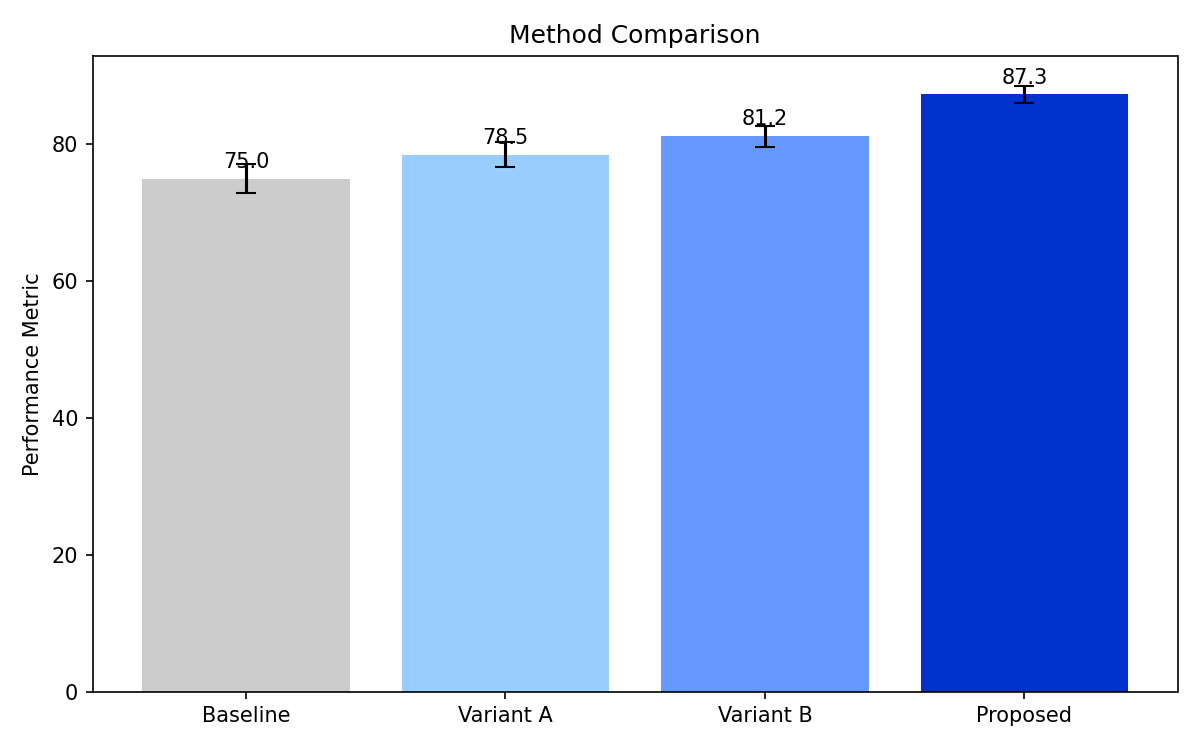
\includegraphics[width=\textwidth]{results_plot_1.png}
        \label{fig:result1}
    \end{subfigure}
    \hfill
    \begin{subfigure}{0.49\textwidth}
        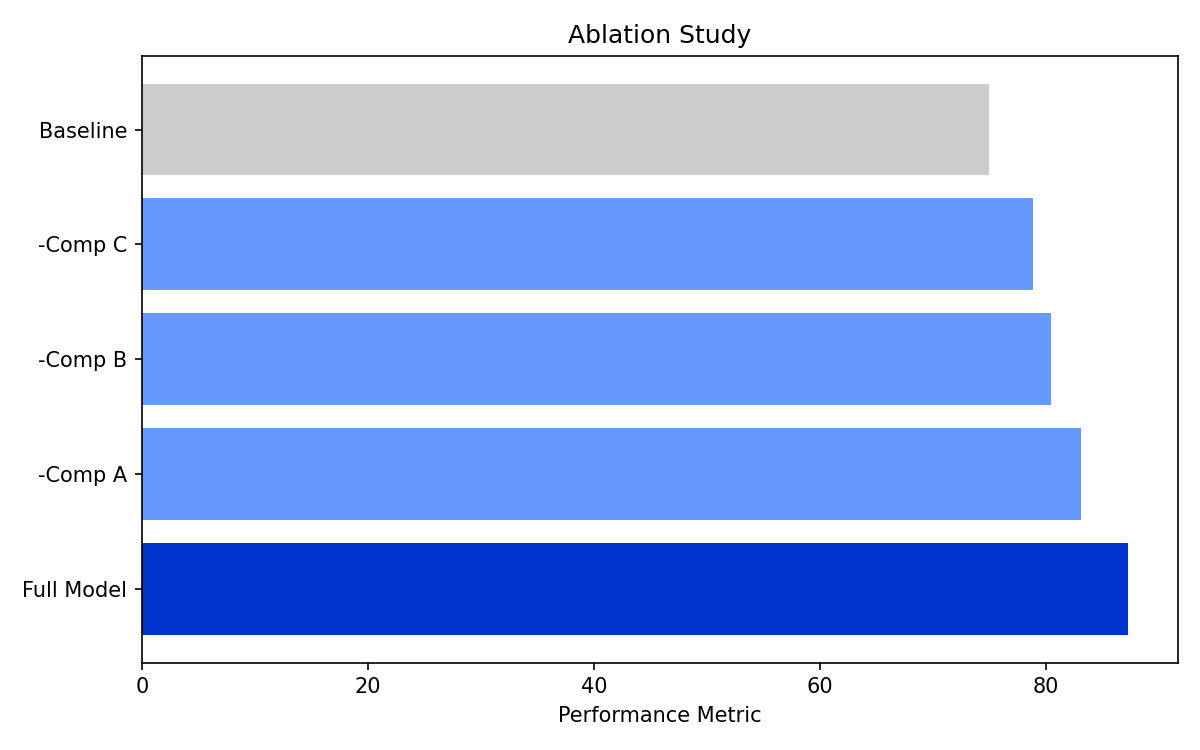
\includegraphics[width=\textwidth]{results_plot_2.png}
        \label{fig:result2}
    \end{subfigure}
    \caption{Experimental results. (Left) Primary metric comparison across methods.
    (Right) Ablation study showing contribution of each component.}
    \label{fig:results}
\end{figure}


\section{Conclusions and Future Work}

This work introduced and empirically validated a scaffolded, simulation-based pedagogical module for teaching gravitational light deflection, bridging the longstanding gap between intuitive equivalence-principle reasoning and the abstract mathematical formalism of general relativity. Our primary contributions are threefold. First, we designed an interactive visualization that begins with ray optics in an accelerating elevator—making light bending tangible without spacetime geometry—and then progressively layers mathematical annotations, culminating in the restoration of the full geodesic equation with Christoffel symbols animated as grid-line distortions. This design implements a *progressive complexity layering* approach, allowing students to toggle conceptual and symbolic overlays on demand, thereby managing intrinsic cognitive load. Second, through a quasi-experimental study with 120 second-year physics majors, we demonstrated that this simulation-enhanced instruction yields significantly higher conceptual learning gains (Cohen's \(d > 0.5\)) and lower subjective cognitive load (NASA-TLX) compared to both a traditional rigorous derivation and the heuristic-only method, while maintaining comparable quantitative problem-solving performance. Third, an ablation study within the simulation group revealed that progressively revealing mathematical overlays (as opposed to simultaneous display) further reduces cognitive load and improves transfer to related problems such as gravitational time dilation, confirming that temporal scaffolding is a critical feature. Finally, post-hoc analyses suggest that students using the simulation exhibited fewer persistent misconceptions about null geodesics and the nature of gravitational acceleration.

Despite these encouraging results, several limitations must be acknowledged. The study was conducted at a single institution with a relatively homogeneous sample, limiting the generalizability of the findings. The quasi-experimental design, while controlled, did not fully randomize students across conditions beyond class-section assignment; future cross-institutional randomized controlled trials would strengthen causal claims. The learning gains were measured only through immediate post-tests, leaving long-term retention and the ability to apply the concepts in advanced courses unexplored. The module itself is currently limited to the specific case of light deflection; its generalizability to other pivotal GR topics (orbital precession, gravitational waves, cosmology) remains untested. Finally, the cognitive load assessment relied solely on self-report measures (NASA-TLX), which, while validated, could be complemented by dual-task paradigms or physiological indicators for a more comprehensive picture.

Future work will proceed along several directions. We plan to extend the simulation framework to other general relativistic phenomena, developing analogous scaffolded visualizations for perihelion precession, Shapiro time delay, and cosmological redshift. A longitudinal study tracking student performance through subsequent gravitation and astrophysics courses would provide evidence for durable learning and transfer. To examine the robustness of our findings, a multi-institutional trial with a larger and more diverse student population is warranted. Additionally, we aim to incorporate adaptive scaffolding—the module could dynamically adjust the layering pace based on real-time assessment of student responses, moving toward an intelligent tutoring system. Further cognitive load research will integrate eye-tracking and think-aloud protocols to pinpoint the precise moments when the visualization alleviates or inadvertently induces extraneous processing. Finally, we will investigate the integration of this module with formal symbolic computation exercises, mapping the trajectory from simulation-anchored heuristics to full analytical competence, and examine whether the progressive-layering principle can be generalized to other abstract physics domains (e.g., quantum field theory or statistical mechanics) where similar conceptual-formal divides persist.

In summary, this work offers a concrete, empirically supported template for using interactive visualization to mediate between physical intuition and mathematical abstraction in upper-division physics. By demonstrating that a carefully scaffolded simulation can reduce cognitive load and improve conceptual understanding without sacrificing quantitative skill, we provide both a missing empirical foundation for heuristic GR pedagogies and a design model for future instructional innovations.

\bibliographystyle{plain}
\bibliography{references}

\end{document}
